\documentclass[chapterprefix=false, 12pt, a4paper, oneside, parskip=half, listof=totoc, bibliography=totoc, numbers=noendperiod]{scrbook}

\usepackage[utf8]{inputenc}
\usepackage[T1]{fontenc}
\usepackage[bottom=48mm,left=25mm,right=25mm]{geometry}
\usepackage[onehalfspacing]{setspace}
\usepackage[stretch=10]{microtype}
\usepackage{xcolor}
\usepackage{scrhack}
\usepackage{titling}
\usepackage[outputdir=out]{minted}
\usepackage{graphicx}
\usepackage{hyperref}
\usepackage[ngerman]{babel}
\usepackage{biblatex}


\renewcommand*{\chapterheadstartvskip}{\vspace*{.25\baselineskip}}
\def\changemargin#1#2{\list{}{\rightmargin#2\leftmargin#1}\item[]}
\let\endchangemargin=\endlist

\definecolor{htwgruen}{RGB}{118, 185, 0}
\definecolor{htwblau}{RGB}{0, 130, 209}
\definecolor{htworange}{RGB}{255, 95, 0}
\definecolor{htwgrau}{RGB}{175, 175, 175}

\title{Bericht über Werkstudententätig bei der DERICON GmbH}
\author{Christoph Stach}
\date{01.11.2016 bis 30.09.2018}

\addbibresource{main.bib}
\defbibheading{none}[\bibname]{
%%
}

\begin{document}
    \begin{titlepage}
        % Logo
        
\includegraphics[width=0.50\textwidth]{img/Q01_HTW_Berlin_Logo_quer_pos_FARBIG_CMYK.eps}

        % Abstand nach logo
        \vspace{4.0cm}

        % Textkörper
        \begin{changemargin}{0.5cm}{0.0cm}
            % Dokumenttyp
            \color{htwgrau}
            \normalsize
            \textsf{\noindent\MakeUppercase{Dokumenttyp}} \vspace{-20pt}\\
            % Horizontale Linie
            \noindent\rule{\textwidth}{0.5pt}\vspace{-4pt}
            % Title
            \color{black}
            \huge
            \textsf{Bericht über Werkstudententätig}
            \vspace{12pt}

            % Author
            \color{htwgrau}
            \normalsize
            \textsf{\MakeUppercase{Author}}\\
            \color{black}
            \large
            \textsf{\theauthor}

            % Zeitraum
            \color{htwgrau}
            \normalsize
            \textsf{\MakeUppercase{Zeitraum}}\\
            \color{black}
            \large
            \textsf{\thedate}

            % Am Ende der Seite
            \vfill

            % Firma
            \color{htwgrau}
            \normalsize
            \textsf{\MakeUppercase{Firma}}\\
            \color{black}
            \large
            \textsf{DERICON GmbH}

            % Dozent
            \color{htwgrau}
            \normalsize
            \textsf{\MakeUppercase{Dozent}}\\
            \color{black}
            \large
            \textsf{Prof. Dr. Schüler}
            \vspace{-60pt}
        \end{changemargin}
    \end{titlepage}

    \tableofcontents

    \chapter{Allgemeines}

    Dieser Bericht behandelt die Werkstudententätigkeit von Christoph Stach bei der DERICON GmbH im Zeitraum vom 01.10.2016 bis 31.09.2018.

    \section{Beschreibung des Unternehmens}

    Die DERICON GmbH ist ein bankenunabhängiges Finanzdienstleistungsinstitut mit Standorten in Frankfurt am Main und Berlin.
    Das Unternehmen unterstützt seit 2008 Banken und Vermögensverwalter bei der Gestaltung effizienter und rechtskonformer Beratungs- und Vertriebsprozesse.
    Mit DERIFIN betreibt DERICON dafür die führende Webanwendung zur Selektion, Steuerung und Risikomanagement von strukturierten Produkten.
    Zudem liefert DERICON professionelle Daten und Kennzahlen für die Analyse und den Einsatz strukturierter Produkte.
    Europaweit vertrauen bereits mehr als 60 Privatbanken, Sparkassen und Genossenschaftsinstitute auf die Expertise von DERICON.
    \\ \\
    Im Jahr 2015 wurde über DERIFIN ein Anlagevolumen von rund 1,2 Mrd. Euro vermittelt.

    \section{Beschreibung der Produkte}

    Das Hauptprodukt von DERICON ist die Webanwendung DERIFIN. Außerdem wurde während ich bei der DERICON GmbH eingestellt war,
    eine neue Version von DERIFIN entwickelt, das sogennante DERIFIN WMS. Welches mehr Features bietet und mit neueren Technologien entwickelt wurde.
    Neben der Hauptsoftware DERIFIN entwickelt DERICON viele internete Produkte zur besseren Verwaltung von DERIFIN und seiner Kunden.

    \section{Beschreibung des Teams}

    Das Team von DERICON ist auf zwei Standorte verteilt. Der erste Standort ist in Frankfurt am Main und der zweite Standort in Berlin Charlottenburg.
    Mein Arbeitsplatz ist im Berliner Büro. Zum heutigen Zeitpunkt arbeiten zwei Frontend-Entwickler, sowie einer der Geschäftsführer in diesem Büro.
    Im Frankfurter Büro arbeiten überwiegend Backend-Entwickler sowie ein weiterer Geschäftsführer und die Buchhaltung.
    \\ \\
    Die komplette Entwicklungsabteilung hält jeden Morgen ein Meeting per Videotelefonie, in dem jedes Mitglied kurz berichtet
    was er am Vortag gemacht hat und was er an diesem Tag vorhat.
    Die Entwicklung ist in Sprints von zwei Wochen gegegliedert. Deswegen gibt es ein weiteres Sprintplanungsmeeting am Anfang eines jeden Sprints.
    Dieser Prozess ist an SCRUM\footnote{Eine Methode für agiles Projektmanagement.} angelehnt.

    \section{Organisation}

    \subsection{Issue-Management}

    Die Aufgabenverteilung ist über die Software JIRA\footnote{Eine Webanwedung für das Projektmanagement und die Fehlerverwaltung von Software. \\ Link: \url{https://www.atlassian.com/software/jira}} geregelt.
    Alle neuen Features sowie anfallende Bugs werden hier gespeichert.
    Bei der Sprintplanung wird besprochen welche Issues\footnote{In JIRA werden Fehler, Features und andere Artefakte generell als Issues bezeichnet.}
    im kommenden Sprint umgesetzt werden sollen. Die Issues werden über den Sprint hinweck vom Teamleader an die einzelnen Entwickler verteilt. Auch ist es möglich sich selbst Issues zuzuweisen.

    \pagebreak

    \subsection{Versionskontrolle}

    Alle Software Projekte werden auf in gespeichert GIT-Repositories\footnote{Eine Versionskontrollsystem entwickelt von Linus Torvalds. Link: \url{https://git-scm.com}} \\
    auf \url{https://bitbucket.org} verwaltet.
    Wird ein Issue aus JIRA von einem Entwickler fertiggestellt, wird auf Bitbucket ein Pullrequest auf den Development-Branch erstellt.
    Dieser muss erst von anderen Entwicklern überprüft werden, bevor er in entgültig in den Development-Branch der Software
    gemerged wird.

    \subsection{Buildmanagement}

    Alle Applikationen werde über JENKINS\footnote{Ein Server zur Automatisierung von Aufgaben, wird oft für den Build-Prozess von Software eingesetzt. Link: \url{https://jenkins.io}} gebaut,
    treten keine Fehler auf beim Buildprozess auf, werden diese danach von JENKINS auf die Server bei Amazon AWS\footnote{Hostingservice für Server und andere Services der Firma Amazon. Link: \url{https://aws.amazon.com}} kopiert.

    \chapter{Aufgaben}

    Während meiner Zeit bei der DERICON GmbH habe ich überwiegend an drei verschiedenen Softwareprodukten gearbeitet.
    Meine Arbeit bezog sich meistens auf die Implementierung neuer Features und dem Beheben von Fehlern. In den Unterpunkten *Entwicklung*
    werde ich jeweils ein paar JIRA-Issues mit einer kurzen Beschreibung referenzieren.

    \section{CitrusNG}

    \subsection{Ausgangsposition}

    CitrusNG war das erste Projekt an dem ich mitgewirkt habe. Es ist ein internes Produkt für die Konfiguration der unterschiedlichen DERIFIN umgebungen, die
    vom Kunden benutzt werden. Jeder Kunde hat unterschiedliche Wünsche deswegen ist die DERIFIN Software sehr stark konfigurierbar, um die Konfigurationen einfacher
    zu verwalten gibt es CitrusNG.

    CitrusNG ist eine Webanwendung. Das Frontend ist mit AngularJS (Version 1)\footnote{JavaScript Framework für die erstellung von Single Page Apps. Link: \url{https://angularjs.org}} implementiert.
    Das Backend mit SpringBoot\footnote{Java Framework der Firma Pivotal. Link: \url{http://spring.io/projects/spring-boot}} Micro-Services.
    Zwischen Backend und Frontend wird eine weitere PHP-Ebene, mit Symfony\footnote{Symfony ist ein weitverbreitetes PHP Framework mit wiederverwendtbaren Bibliotheken und Komponenten der Firma SensioLabs. Link: \url{https://symfony.com}}
    implementiert, in Form einer Middleware eingesetzt. Die Middleware sowie das Frontend wird von den Frontent-Entwicklern gepflegt.
    Das Ziel der Middleware ist es den Frontend-Entwicklern die Möglichkeit zu geben, die Ergebnisse der
    Backend-Endpunkte zu manipulieren und sie angepasst an das Frontend weiterzuleiten. 
    Hier werden beispielsweise unötige JSON\footnote{JavaScript Object Notation: Ein Format für die Übertragung von Objekten zwischen Server und Client Anwendungen}-Felder entfernt oder
    aggregiert, Mock-Daten generiert oder Sortierfunktionen implementiert.

    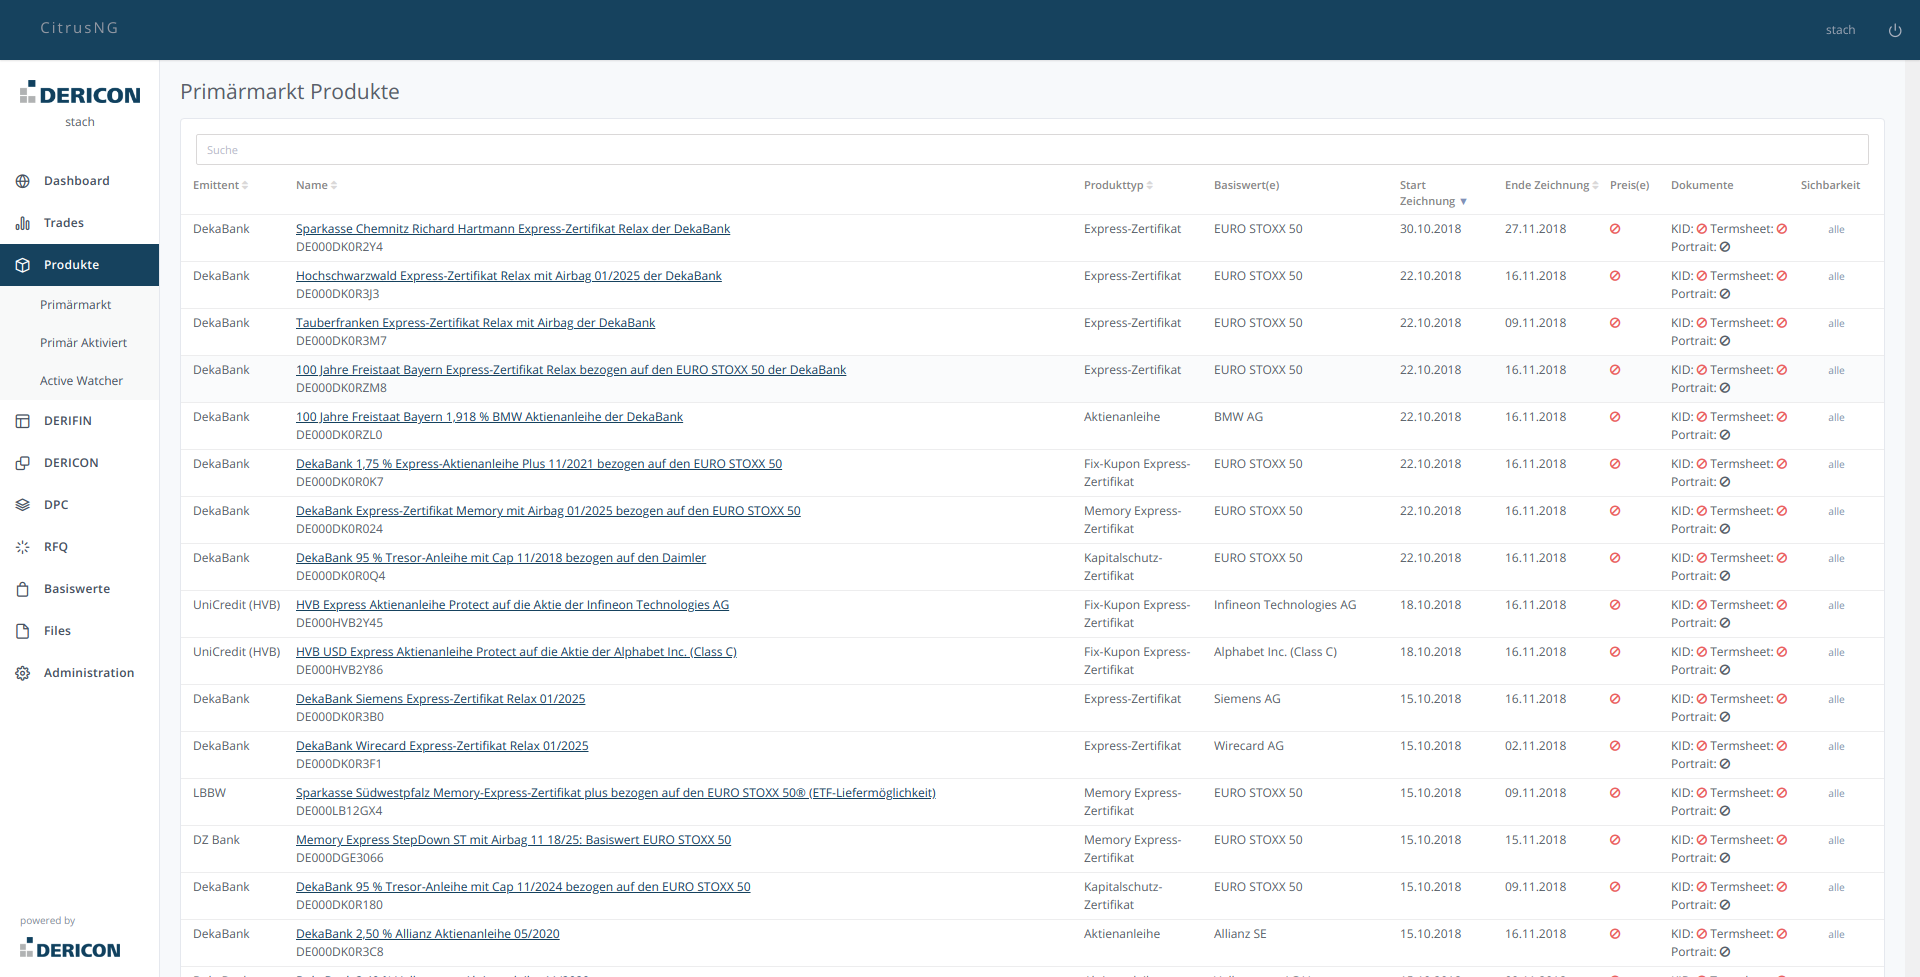
\includegraphics[width=1.00\textwidth]{img/citrusng.png}
    \captionof{figure}{Screenshot der Software CitrusNG}

    \subsection{Entwicklung}

    An CitrusNG habe ich unterschiedliche Aufgaben vollrichtet. Ich habe insgesamt ca. 1 Jahr an diesem Projekt mitgewirkt.

    Beispiele meiner Arbeit:

    \textbf{CNG-319: Möchten Sie wirklich die Seite verlassen, Sie haben noch ungespeicherte Änderungen}

    Es sollte bei diesem Feature eine Bestätigung angezeigt werden, welche angezeigt wird wenn bereits Änderungen an einem Formular
    gemacht worden sind und diese vom Benutzer nicht gespeichert wurden bevor er die Seite verlässt.

    Sobald Änderungen am Formular vorliegen muss eine Variable \textit{vm.saved} auf \textit{false} gesetzt werden.

    \begin{minted}[xleftmargin=20pt,linenos,breaklines]{javascript}
    function changed() {
        vm.saved = false;
    }
    \end{minted}

    Außerdem muss die Variable \textit{\$scope} überwacht werden. Darüber kann bei AngularJS überprüft werden ob der
    Benutzer die aktuelle Seite verlassen will und man kann auf dieses Ereignis reagieren.

    \begin{minted}[xleftmargin=20pt,linenos,breaklines]{javascript}
    function DividendsController(apiClient, \$q, \$state, \$scope) {
        var vm = this;
        vm.saved = false;

        function onStateChange(event, toState, toParams) {
            if (!vm.saved) {
                if (!confirm('Wollen Sie die Seite wirklich verlassen? Ungespeicherte Änderungen gehen verloren!')) {
                    event.preventDefault();
                }
            }
        }
    }
    \end{minted}

    \textbf{CNG-381: DPC Emittierte Produkte - Liste sortierbar machen}

    In diesem Issue sollte, wie der Titel sagt, eine Tabelle von Produkten sortierbar gemacht werden.
    Die zu dem Zeitpunkt bereits bestehende Tabelle benutzt das AngularJS-Plugin Smart Table\footnote{Link: \url{http://lorenzofox3.github.io/smart-table-website/}}.
    Das Plugin bietet die Möglich einfach dynamisch generierte Tabellen zu erstellen. Es außerdem bietet Angular Directive um die Tabellen-Spalten sortierbar zu machen.

    \begin{minted}[xleftmargin=20pt,linenos,breaklines]{html}
    <th>
        <div st-sort="environmentData.name" class="th-label">
            Umgebung Name <i class="fa fa-sort"></i>
        </div>
    </th>
    \end{minted}

    Zur Umsetzung der Aufgabe habe ich lediglich die entsprechende \textit{st-sort} Directive zu den zu sortierenbaren Spalten sowie ein Sortier-Icon hinzugefügt.
    Der Wert der Directive entspricht dem Key im JavaScript-Objekt nach dem sortiert werden soll.

    \subsection{Ergebnisse}

    Während meiner Arbeit an CitrusNG habe ich insgesamt 40 JIRA-Issues bearbeitet. Dabei handelte
    es sich um das Beheben von Fehlern in der Software sowie auch der Implementierung neuer Features.

    \section{BrokerUI}

    \subsection{Ausgangsposition}

    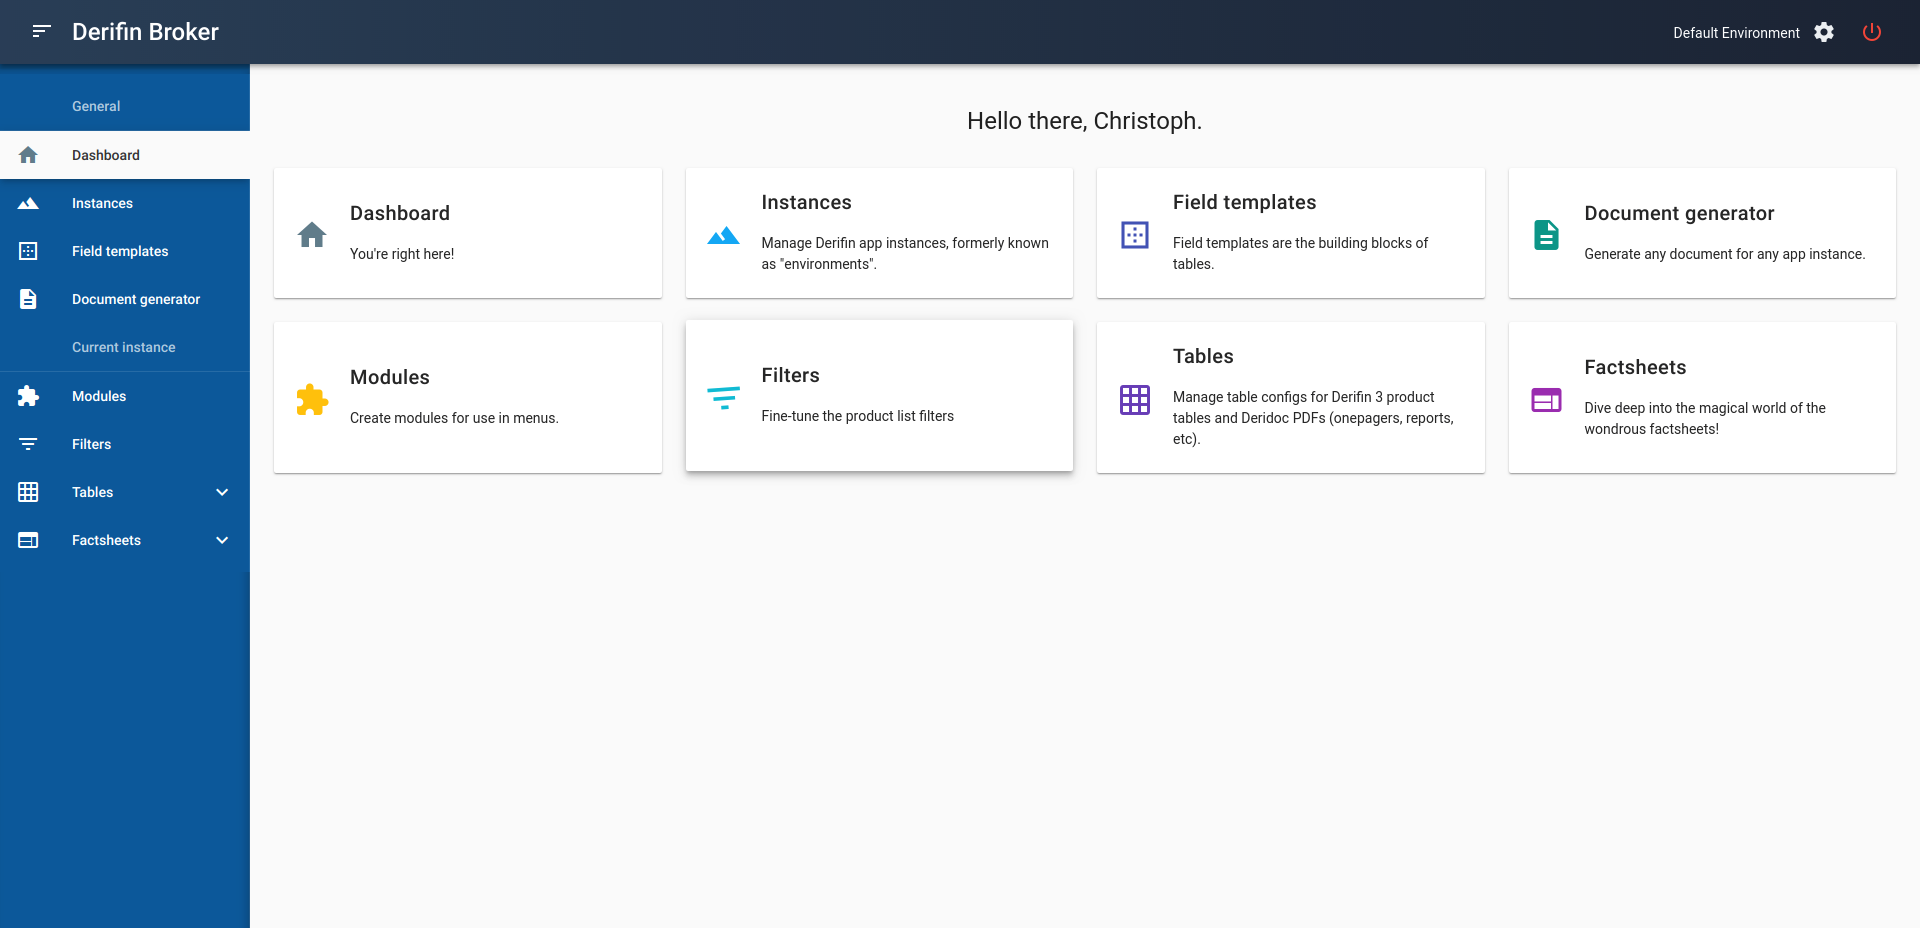
\includegraphics[width=1.00\textwidth]{img/broker-ui-neu.png}
    \captionof{figure}{Screenshot der Software BrokerUI}


    \subsection{Entwicklung}

    \subsection{Ergebnisse}

    \section{DERIFIN WMS}

    \subsection{Ausgangsposition}

    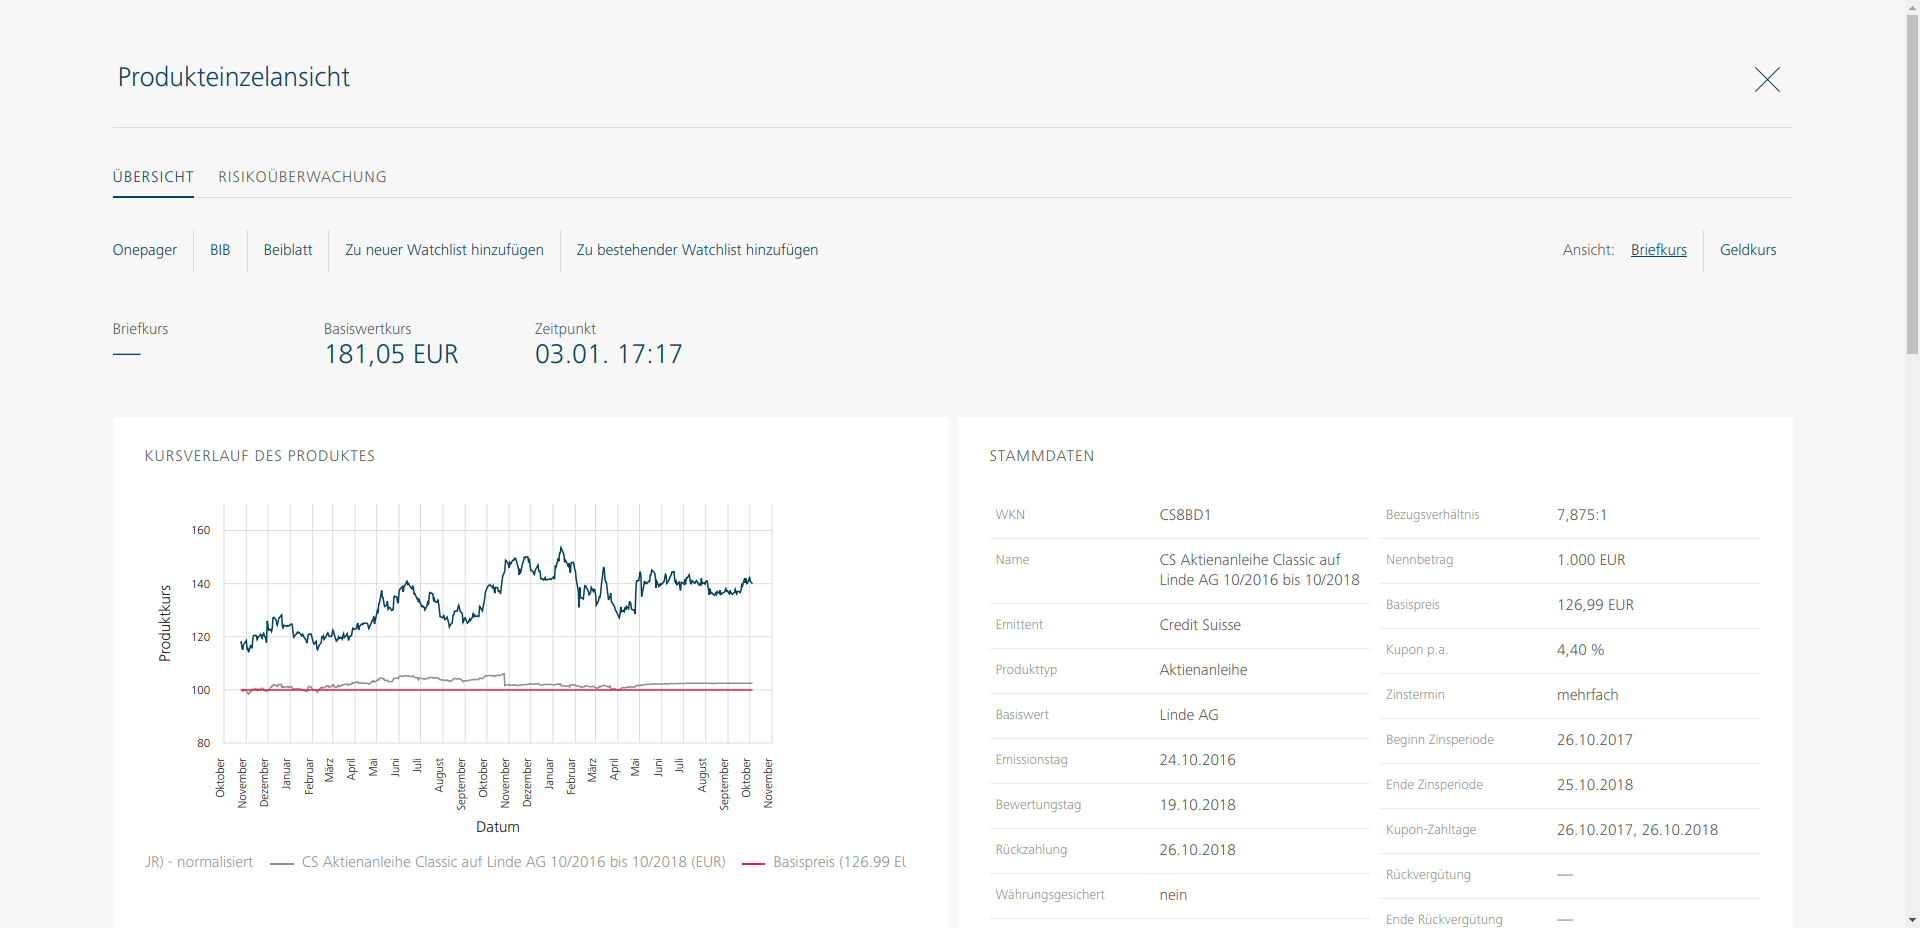
\includegraphics[width=1.00\textwidth]{img/derifin.png}
    \captionof{figure}{Screenshot der Software DERIFIN WMS}

    \subsection{Entwicklung}

    \subsection{Ergebnisse}

    \chapter{Schlussfolgerungen}

    \section{Zusammenhänge mit dem Studium an der HTW Berlin}

    Durch meine Arbeit bei der DERICON GmbH konnte ich mein Wissen, besonders im Bereich der Webentwicklung, erweitern.
    Ich konnte viele Ansätze die im Modul \textit{Webentwicklung} an der HTW  Berlin geleehrt wurden anwenden. Ich habe die zwei Frameworks
    AngularJS und Angular kennengelernt. Besonders mit der Arbeit mit Angular konnte ich Parallelen zum Studium ziehen. Angular
    verwendet verstärkt Bibliothek \textit{rxjs}, welche das Observable-Pattern implementiert. Dieses wurde bereits im Modul
    \textit{Programmierung 3} an der HTW Berlin behandelt. Außerdem wird viel mit Functional Programming Methoden gearbeitet die auch bereits in Form
    von Streams in \textit{Programmierung 3} sowie im Modul \textit{Entwicklung sozialer Anwendungen} geleehrt wurden.

    Bei meiner Arbeit an der Software \textit{CitrusNG} habe ich viel mit dem MVC-Paradigma gearbeitet. Dieses wird bei \textit{Symfony}
    und \textit{AngularJS} viel verwendet. Dadurch konnte ich Verbindungen zu den Modulen \textit{Webentwicklung} und \textit{Programmierung 3}
    sowie \textit{Software Engineering} herstellen.

    \chapter{Anhang}

    \section{Literaturverzeichnis}

    \printbibliography[heading=none]

    \section{Glossar}
\end{document}
